\begin{figure}[h!]
\begin{center}
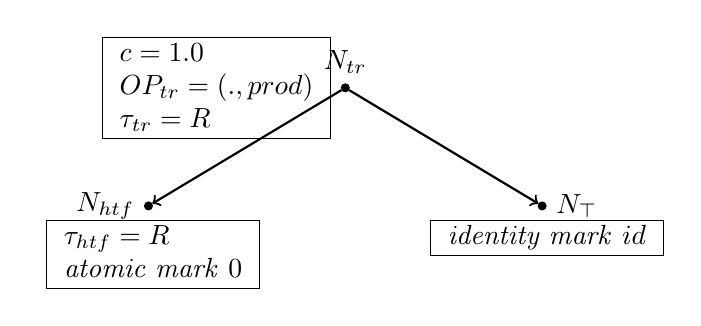
\begin{tikzpicture}[yscale=-1,
place/.style={circle,draw=black, fill=black, inner sep=0pt, 
              minimum size=1mm}]

  \node[place] (1st) at (2.5, 0) [label=above: $N_{tr}$,
                                  label=left: { 
             \begin{tabular}{|l|}
               \hline
               $c=1.0$\\
               $OP_{tr}=(.,prod)$\\
               $\tau_{tr}=R$\\
               \hline
             \end{tabular} }
] {};
	\node[place] (2nd) at (0, 1.5) [label=left: $N_{htf}$,
                                        label=below: {
              \begin{tabular}{|l|}
                \hline
                 $\tau_{htf}=R$ \\
                 \textit{atomic mark} $0$ \\
                \hline
              \end{tabular} }
             ] {};

        \node[place] (3rd) at (5, 1.5) [label=right: $N_{\top}$, 
                                        label=below: {
              \begin{tabular}{|l|}
               \hline
               \textit{identity mark} $id$ \\
               \hline
              \end{tabular} }
] {}; 

	\draw[->, thick] (1st) -- (2nd);
        \draw[->, thick] (1st) -- (3rd);
\end{tikzpicture}
\end{center}
\caption{Expansion of tr}
\label{fig:ExpansionTr}   
\end{figure}